\documentclass[border=4pt]{standalone}
\usepackage{tikz}
\usetikzlibrary{shapes.symbols,positioning,arrows.meta}

\begin{document}
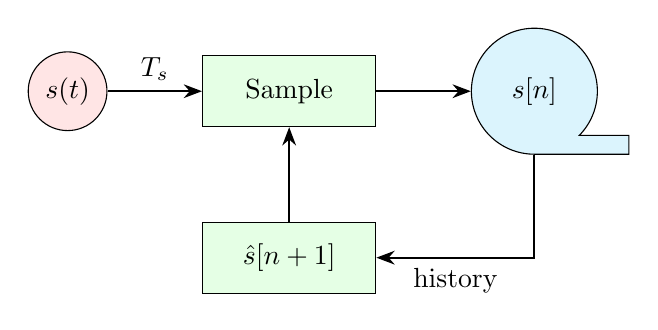
\begin{tikzpicture}[
  >=Stealth,
  node distance=12mm,
  block/.style={draw,minimum width=22mm,minimum height=9mm,fill=green!10},
  tape/.style={magnetic tape,draw,minimum size=16mm,magnetic tape tail=.3,
    magnetic tape tail extend=4mm,fill=cyan!14},
  flow/.style={->,thick}
]
  \node[draw,circle,minimum size=10mm,fill=red!10] (sensor) {$s(t)$};
  \node[block,right=of sensor] (sample) {Sample};
  \node[tape,right=of sample] (record) {$s[n]$};
  \node[block,below=of sample] (model) {$\hat s[n+1]$};

  \draw[flow] (sensor) -- node[above]{$T_s$} (sample);
  \draw[flow] (sample) -- (record);
  \draw[flow] (record.south) |- node[pos=.75,below]{history} (model.east);
  \draw[flow] (model) -- (sample);
\end{tikzpicture}
\end{document}
